
\documentclass[calculator,steamtables,datasheet,solutions]{exam}
%\documentclass[calculator,fluidstables,allquestions,datasheet]{exam}

% The full list of class options are
% calculator : Allows approved calculator use.
% datasheet : Adds a note that data sheet are attached to the exam.
% handbook : Allows the use of the engineering handbook.
% resit : Adds the resit markings to the paper.
% sample : Adds conspicuous SAMPLE markings to the paper
% solutions : Uses the contents of \solution commands (and \solmarks) to generate a solution file

\usepackage{pdfpages} 
\usepackage{lscape,comment}
 
\coursecode{EX3029}%%

\examtime{09.00--12.00}%
\examdate{03}{03}{2015}% 
\examformat{Candidates must attempt \textit{all} questions.}

\newcommand{\frc}{\displaystyle\frac}
\newcommand{\br}[1]{\!\left( #1 \right)}
\newcommand{\abs}[1]{\left| #1 \right|}
\newcommand{\fracd}[2]{\frac{\mathrm{d} #1}{\mathrm{d} #2}}
\newcommand{\fracp}[2]{\frac{\partial #1}{\partial #2}}
\renewcommand{\d}[1]{\mathrm{d} #1 } 
\newcommand{\Ma}{\mathrm{M\!a}} 



\begin{document}

%%%
%%% Question 01
%%%
\begin{question}
%
\begin{enumerate}[(a)]
%%% Johannes T3Q4
\item Assuming $S = S\left(P,V\right)$ and taking into consideration that,
\begin{displaymath}
\left(\frc{\partial S}{\partial T}\right)_{V} = \frc{C_{V}}{T}\;\;\;\text{ and }\;\;\; \left(\frc{\partial S}{\partial T}\right)_{P} = \frc{C_{P}}{T}
\end{displaymath}
Prove that 
\begin{displaymath}
\d S = \frc{C_{V}}{T}\left(\frc{\partial T}{\partial P}\right)_{V}\d P + \frc{C_{P}}{T}\left(\frc{\partial T}{\partial V}\right)_{P}\d V
\end{displaymath}~\marks{7}
%
\solution{As entropy is expressed as a function of pressure and molar volume, we can write it in differenctial form as,~\solmarks{1/7}
\begin{displaymath}
  dS = \left(\frc{\partial S}{\partial P}\right)_{V}dP + \left(\frc{\partial S}{\partial V}\right)_{p}dV 
\end{displaymath}
We can rewrite this equation as~\solmarks{3/7}
\begin{displaymath}
dS = \left(\frc{\partial S}{\partial T}\right)_{V}\left(\frc{\partial T}{\partial P}\right)_{V}dP + \left(\frc{\partial S}{\partial T}\right)_{p}\left(\frc{\partial T}{\partial V}\right)_{p}dV
\end{displaymath}
As $\left(\frc{\partial S}{\partial T}\right)_{V}=\frc{C_{v}}{T}$ and $\left(\frc{\partial S}{\partial T}\right)_{P}=\frc{C_{P}}{T}$, ~\solmarks{4/7}
\begin{displaymath}
dS = \frc{C_{v}}{T}\left(\frc{\partial T}{\partial P}\right)_{V}dP + \frc{C_{P}}{T}\left(\frc{\partial T}{\partial V}\right)_{p}dV
\end{displaymath}
}


% (Shapiro 2.34) 
\item Air contained in a piston-cylinder system undergoes three consecutive processes,
\begin{itemize} 
\item Process 1--2: Isobaric cooling with P$_{1}$=69 kPa and V$_{1}$=0.11 m$^{3}$;
\item Process 2--3: Isochoric heating with P$_{3}$=345 kPa;
\item Process 3--1: Polytropic expansion, with $PV=$ {\it constant}. %Expansion to the initial state, during which the pressure-volume relationship is $PV=$ {\it constant}.
\end{itemize}  
\begin{enumerate}[(i)]
\item Calculate V$_{2}$ $\left(\text{in m}^{3}\right)$.~\marks{3} 
\solution{
For Process 2--3: V$_{2}$=V$_{3}$. However the expansion 3--1 follows $PV=$ constant,
\begin{displaymath}
P_{1}V_{1}=P_{3}V_{3} \Longrightarrow V_{3} = \frc{P_{1}V_{1}}{P_{3}} = {\bf 0.022\;\text{m}^{3} = V_{2}}
\end{displaymath}~\solmarks{3/3}
}
\item Calculate the work (in $kJ$) for each process.~\marks{6}
\solution{\noindent
Process 1--2: 
\begin{displaymath}
{\bf W_{1-2}} = \int\limits_{V_{1}}^{V_{2}} P dV = P\left(V_{2}-V_{1}\right) = -6072 J \Rightarrow {\bf -6.072 kJ}
\end{displaymath}~\solmarks{2/6}
\noindent
Process 2--3: V$_{2}$=V$_{3}$ $\Longrightarrow$ {\bf W$_{2-3}$ = 0}~\solmarks{2/6} \\
\noindent
Process 3--1: $PV = C$
\begin{displaymath} 
{\bf W_{31}} = \int\limits_{V_{3}}^{V_{1}}P dV = \int\limits_{V_{3}}^{V_{1}}\frc{C}{V} dV = P_{1}V_{1}\ln\frc{V_{1}}{V_{3}} = 12220 J \Rightarrow {\bf 12.22 kJ} 
\end{displaymath}~\solmarks{2/6}
}
\item Sketch the $PV$ diagram for these processes.~\marks{4}
\solution{\solmarks{4/4}
\begin{center}
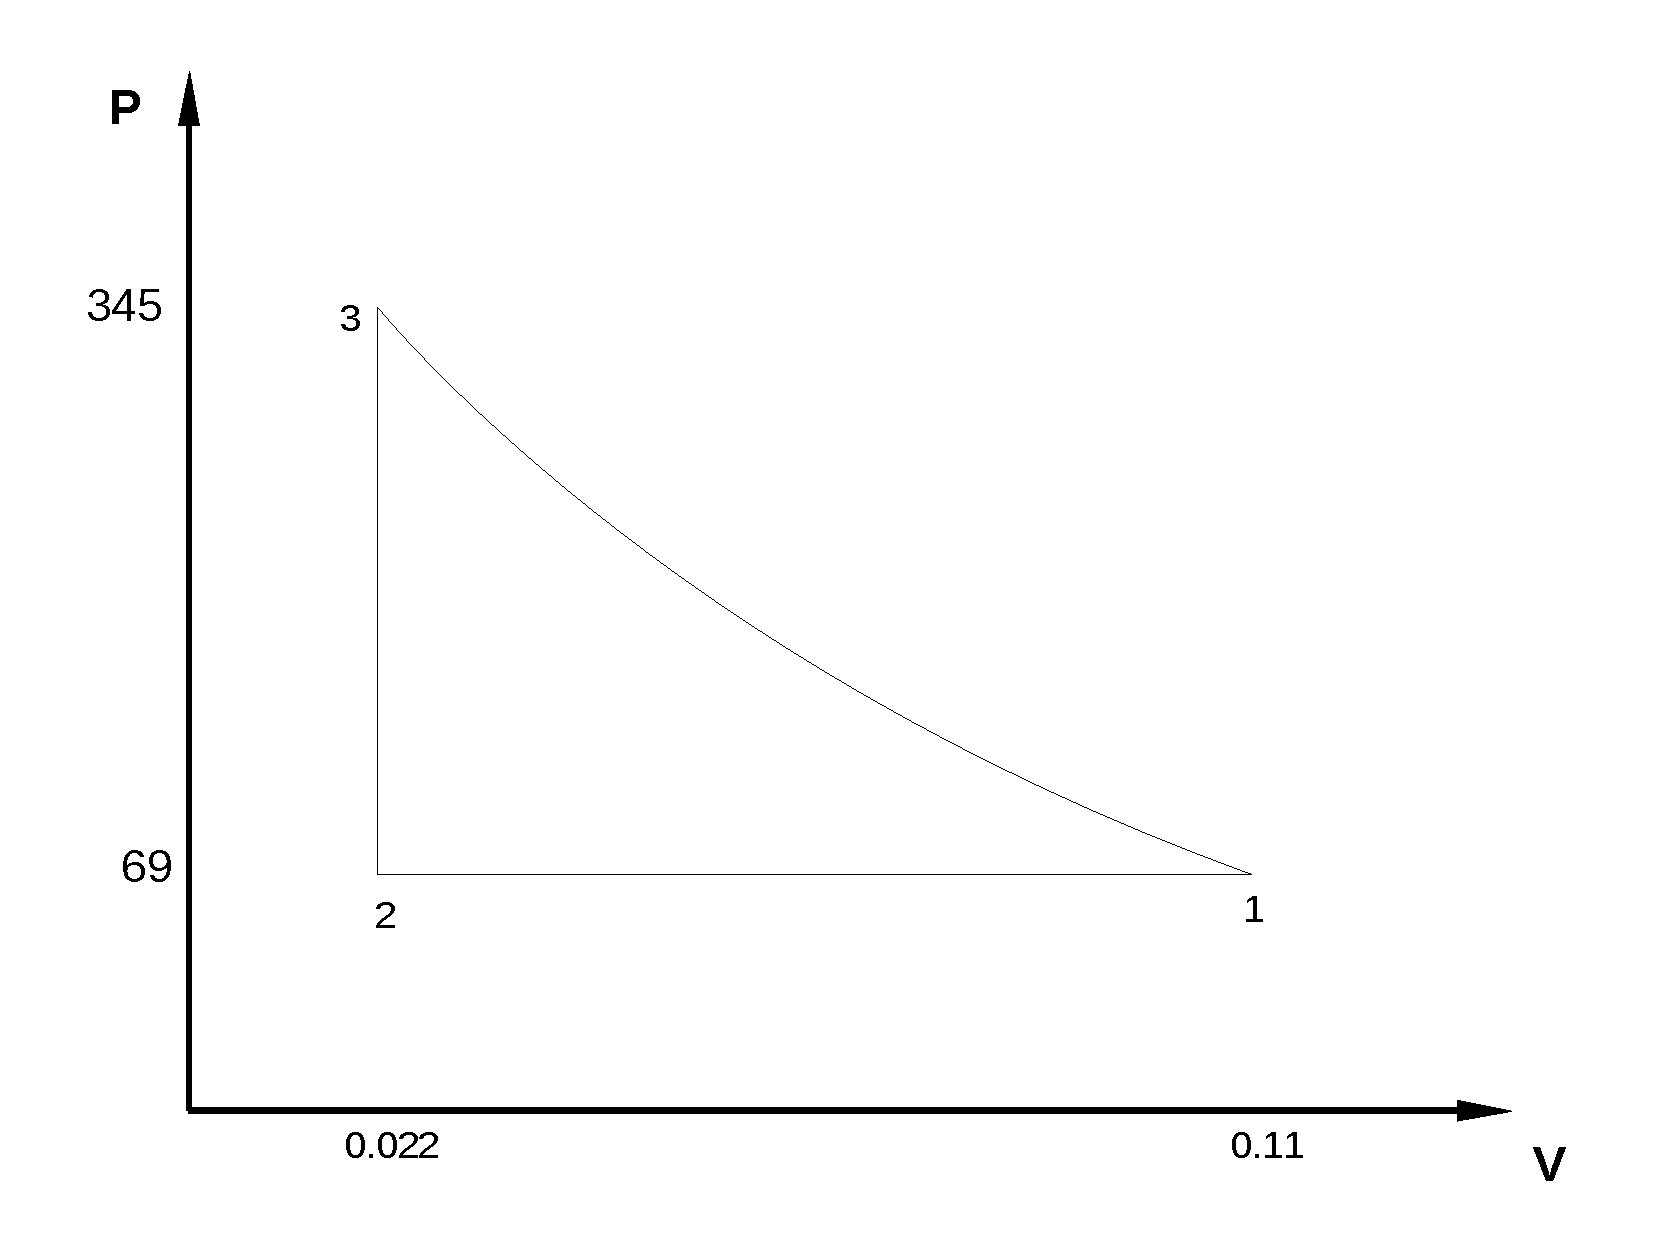
\includegraphics[width=10.cm,height=8.cm,clip]{./Pics/Exam_PV_Diagram}
\end{center}
}
%
\end{enumerate}
%
\end{question}
\clearpage

%%%
%%% Question 02
%%%
\begin{question}
%
\begin{enumerate}[(a)]
%
\item Develop expressions for the volume expansivity, $\beta=\frc{1}{V}\left(\frc{\partial V}{\partial T}\right)_{P}$, and isothermal compressibility, $\kappa=-\frc{1}{V}\left(\frc{\partial V}{\partial P}\right)_{T}$, for the following equations of state,
\begin{enumerate}[(i)]
\item ideal gas~\marks{4}
\solution{Ideal gas: $V=\frc{RT}{P}$,
\begin{displaymath}
\left(\frc{\partial V}{\partial T}\right)_{P} = \frc{R}{P} \;\;\; \left(\frc{\partial V}{\partial P}\right)_{T} = -\frc{RT}{P^{2}} 
\end{displaymath}~\solmarks{2/4}
Now deriving $\beta$ and $\kappa$,
\begin{displaymath}
{\bf \beta} = \frc{1}{V}\frc{R}{P} {\bf = \frc{1}{T}}\;\;\text{ and}\;\;\kappa = -\frc{1}{V}\left(-\frc{RT}{P^{2}}\right){\bf = \frc{1}{P}}
\end{displaymath}~\solmarks{2/4}
}
\item $V=\frc{RT}{P}+b$~\marks{4}
\solution{
The derivatives are,
\begin{displaymath}
\left(\frc{\partial V}{\partial T}\right)_{P} = \frc{R}{P} \;\;\; \left(\frc{\partial V}{\partial P}\right)_{T} = -\frc{RT}{P^{2}} 
\end{displaymath}~\solmarks{2/4}
Now deriving $\beta$ and $\kappa$,
\begin{displaymath} 
{\bf \beta} = \frc{1}{V}\frc{R}{P} =\frc{R}{V}\frc{V-b}{RT}= {\bf = \frc{1}{T}\frc{V-b}{V}} \;\;\text{ and }\;\; {\bf \kappa} = -\frc{1}{V}\left(-\frc{RT}{P^{2}}\right){\bf = \frc{1}{P}\left[\frc{V-b}{V}\right]}
\end{displaymath}~\solmarks{2/4}
}
\end{enumerate}

\item Calculate the compressibility factor ($Z$) and molar volume of sulpher dioxide $\left(SO_{2}\right)$ vapour at 300 K and 4 bar using the Redlich-Kwong equation of state. Properties of SO$_{2}$ are: T$_{c}$ = 430 K, P$_{c}$ = 78.7 bar and $\omega$ = 0.251 (accentric factor). In your iterative calculations, use $Z_{0}=1$ as initial guess of $Z$, and stop at the second iteration $\left(Z_{2}\right)$.~\marks{12}
\solution{ The generic form of $Z$ is,
\begin{displaymath}
Z = 1+ \beta - q\beta\frc{Z - \beta}{\left(Z+\epsilon\beta\right)\left(Z+\sigma\beta\right)}\;\;\text{ with} \;\; \beta = \Omega \frc{P_{r}}{T_{r}}\;\;\text{ and}\;\; q=\frc{\Psi\alpha}{\Omega T_{r}}
\end{displaymath}
For SRK with {\bf T$_{r}$=0.8380}, {\bf P$_{r}$=0.3754}, {\bf $\beta$=3.88$\times$10$^{-2}$} and {\bf $q$=6.7274}~\solmarks{2/12},
\begin{displaymath}
{\bf Z = 1 + \beta - q\beta\frc{Z-\beta}{Z^{2}+\beta Z}}
\end{displaymath}~\solmarks{2/12}
The equation is non-linear and to find the root we can apply Newton-Raphson method 
\begin{displaymath}
Z_{i} = Z_{i-1} - \frc{\mathcal{F}\left(Z_{i-1}\right)}{d\mathcal{F}/dZ \left(Z_{i-1}\right)}
\end{displaymath}
with,
\begin{eqnarray}
&& \mathcal{F}\left(Z\right) = Z - \left[ 1 + \beta - q\beta\frc{Z-\beta}{Z^{2}+\beta Z}\right] \nonumber \\
&& \frc{d\mathcal{F}}{dZ}\left(Z\right) = 1 + q\beta \frc{\beta^{2}+2\beta Z- Z^{2}}{\left(Z^{2}+\beta Z\right)^{2}} \nonumber
%\frc{q\beta\left(Z^{2}\beta +Z\right)-q\beta Z\left(2Z + \beta\right)}{\left(Z^{2}+\beta Z\right)^{2}} + \frc{q\beta^{2}\left(2Z+\beta\right)}{\left(Z^{2}+\beta Z\right)^{2}} \nonumber
\end{eqnarray} 
as initial guess, we can use the generic real gas EOS, $PV=Z_{0}RT \Longrightarrow$ {\bf $Z_{0}=0.7217$}~\solmarks{2/12}. Thus 
\begin{center}
{\bf $Z_{1}$ = 0.7184}~\solmarks{3/12} \\
{\bf $Z_{2}$ = 0.7160}~\solmarks{3/12} \\
$\cdots \cdots \cdots $ \\
\textcolor{red} {or (using calculator) }{\bf $Z_{22}$ = 0.7088}~\solmarks{\textcolor{red}{8/12}} \\

\end{center}
} 
%
\end{enumerate}
%
\end{question}

\clearpage

%%%
%%% Question 03
%%%
\begin{question}
%
\begin{enumerate}[(a)]
%%%
%%% Johannes Lecture Example
%%%
\item\label{LectExample} In the esterification reaction of acetic acid with ethanol at 100$^{\circ}$C,
\begin{displaymath}
CH_{3}COOH + C_{2}H_{5}OH  \Longleftrightarrow  CH_{3}COOC_{2}H_{5} + H_{2}O,
\end{displaymath}
calculate the mass fraction of ethyl acetate given that initially there was 1 mole of acetic acid and ethanol. The reaction enthalpy and Gibbs energy at standard state (25$^{\circ}$C and 1 atm) are $\Delta H_{298}^{\circ}=-3640$ J and $\Delta G_{298}^{\circ}=-4650$ J. Given the van't Hoff equation,~\marks{7}
\begin{displaymath}
\frc{d}{dT}\left(\ln{K}\right) = - \frc{\Delta H_{298}^{o}}{RT^{2}}
\end{displaymath}

%==========================
\solution{ Initially we have 1 mol of acetic acid (HAc) and 1 mol of ethanol (EtOH). We can calculate the mole fractions for all species as a function of the reaction coordinate, $\epsilon$
\begin{eqnarray}
 x_{\text{EtAc}} &=& \frc{\epsilon}{2+0.\epsilon} = \frc{\epsilon}{2} = x_{H_{2}O}  \nonumber \\
 x_{\text{HAc}} &=& \frc{1-\epsilon}{2} = x_{\text{EtOH}} \nonumber
\end{eqnarray}
Assuming ideal solution,~\solmarks{1/7}
\begin{displaymath}
  \prod\limits_{i=1}^{c=4} x_{i}^{\nu} = K = x_{\text{HAc}}^{-1}\;x_{\text{EtOH}}^{-1}\;x_{\text{EtAc}}\;x_{H_{2}O} \Longrightarrow K = \frc{\epsilon^{2}}{\left(1-\epsilon\right)^{2}}
\end{displaymath} 
Thus, by calculating $K$, we can obtain $\epsilon$ and then $x_{\text{EtAc}}$. $K$ (temperature-dependent) can be obtained from the Gibbs free energy,~\solmarks{2/7}
\begin{displaymath}
   \ln{K_{298}} = -\frc{\Delta G_{298}^{o}}{RT} = \frc{4650.0}{8.314\times 298.15} = 1.8759
\end{displaymath}
Now, in order to calculate $K$ at 373.15 K, we can integrate the van't Hoff equation from 298.15 K to 373.15 K~\solmarks{2/7}
\begin{displaymath}
\int\limits_{K_{298}}^{K_{373}} d\left(\ln{K}\right) = - \int\limits_{298.15}^{373.15}\frc{\Delta H_{298}^{o}}{RT^{2}} dT \Longrightarrow K_{373} = 4.8586
\end{displaymath}
Now we can calculate the reaction coordinate,
\begin{displaymath}
   K_{373} = \frc{\epsilon^{2}}{\left(1-\epsilon\right)^{2}} \Longrightarrow \epsilon= 0.6879
\end{displaymath} 
Thus ~\solmarks{2/7}
\begin{displaymath}
x_{\text{EtAc}} = \frc{\epsilon}{2} = 0.3440
\end{displaymath}

 }

%%%
%%% Johannes T0902
%%%
\item\label{T0902} Assuming that all species and their mixtures are ideal gases, derive an equation for the Gibbs energy as a function of the reaction coordinate for the reaction below at 1000K.
\begin{displaymath}
H_{2} + CO_{2} \Longleftrightarrow H_{2}O + CO
\end{displaymath}
Given $\Delta G_{f}^{\circ}$ $\left(\text{J.gmol}^{-1}\right)$ at 1000K: (a) H$_{2}$O: -192420, (b) CO: -200240 and (c) CO$_{2}$: -395790.~\marks{13}
\solution{ hjhu }
%
\end{enumerate}
%
\end{question}

\clearpage

%%%
%%% Question 04
%%%
\begin{question}
%
\begin{enumerate}[(a)]
%%%
%%% Jeff Solved Example 3 ==> Sandler Example 10.1.4 (page 504)
%%%
\item\label{Example_03} An ideal liquid mixture of 25 mol-$\%$ n-pentane $\left(nC_{5}\right)$, 45 mol-$\%$ n-hexane $\left(nC_{6}\right)$ and 30 mol-$\%$ n-heptane $\left(nC_{7}\right)$, initially at 69$^{\circ}$C and high pressure, is partially vaporised by isothermically lowering the pressure to 1.013 bar. Calculate the relative amounts of vapour and liquid in equilibrium and their compositions.~\marks{10}
\solution{90k}

%%%
%%% Jeff Solved Example 2 ==> Sandler Example 10.1.2 (page 501)
%%%
\item Estimate the bubble point temperature of a 25 mol-$\%$ n-pentane $\left(nC_{5}\right)$, 45 mol-$\%$ n-hexane $\left(nC_{6}\right)$ and 30 mol-$\%$ n-heptane $\left(nC_{7}\right)$ mixture at 1.013 bar.~\marks{10}
\solution{ iouh} 
%
\end{enumerate}

For This problem, use 
\begin{displaymath}
   \ln P_{i}^{\text{sat}} = A_{i} - \frc{B_{i}}{RT}
\end{displaymath} 
with [P] = bar and [T] = K, and
    \begin{center}
       \begin{tabular}{l l l} 
          $A_{nC_{5}}=10.422$ & $A_{nC_{6}}=10.456$ & $A_{nC_{7}}=11.431$ \\
          $B_{nC_{5}}=26799$  & $B_{nC_{6}}=29676$  & $B_{nC_{7}}=35200$  
       \end{tabular}
    \end{center}
%
\end{question}

\clearpage

%%%
%%% Question 05
%%%
\begin{question}
%
\begin{enumerate}[(a)]

%%%
%%% Johannes Problem 2 (Tutorial 5)
%%%
\item\label{Tut05P2} A process stream contains light species 1 and heavy species 2. A relatively pure liquid stream containing mostly 2 is obtained through a single-stage liquid/vapour separator. Specifications on the equilibrium composition are: $x_{1}$ = 0.002 and $y_{1}$ = 0.950. Assuming that the modified Raoult's law applies, 
\begin{displaymath}
  y_{i} P = x_{i}\gamma_{i}P_{i}^{\text{sat}}
\end{displaymath} 
Determine $T$ and $P$ for the separator. Given the activity coefficients for the liquid phase,~\marks{20}
\begin{displaymath}
\ln\gamma_{1} = 0.93x_{2}^{2} \;\;\;\;\;\text{ and }\;\;\;\;\;\ln\gamma_{2}=0.93x_{1}^{2}
\end{displaymath}
\begin{displaymath}
\ln P^{\text{sat}} = A - \frc{B}{T}\;\;\;\text{with [P] = bar and [T] = K}
\end{displaymath} 
$A_{1}$ =10.08, $B_{1}$ = 2572.0, $A_{2}$ = 11.63 and $B_{2}=6254.0$.

\end{enumerate}

\end{question}



\clearpage

%%%
%%% Question 06
%%%
\begin{question}
%
\begin{enumerate}[(a)]

%%% Johannes T0602
%%%
\item\label{T0602} What is the change in entropy when 700 litres of CO$_{2}$ and 300 litres of N$_{2}$, each at 1 bar and 25$^{\circ}$C blend to form a gas mixture at the same conditions? Assume ideal gases, and given~\marks{6}
\begin{displaymath}
\Delta S = - nR\sum\limits_{i=1}^{n}y_{i}\ln{y_{i}}
\end{displaymath}


%%%
%%% SM &VN 11.13
%%%
\item\label{Ex2} The molar volume $\left(\text{in cm}^{3}\text{.gmol}^{-1}\right)$ of a binary liquid mixture at $T$ and $P$ is given by:
\begin{displaymath}
V = 120 x_{1} + 70 x_{2} + \left( 15x_{1} + 8x_{2}\right)x_{1}x_{2} 
\end{displaymath}
\begin{enumerate}
\item\label{first} Find expressions for the partial molar volumes of species 1 and 2 at $T$ and $P$.
\item Show that when these expressions are combined in accord with $M=\sum\limits_{i}x_{i}\overline{M}_{i}$, the given equation for $V$ is recovered;
\item Show that these expressions satisfy the Gibbs-Duhem equation, $\sum\limits_{i}x_{i}d\overline{M}_{i}=0$;
\item Show that 
   \begin{displaymath}
        \left(\frc{d\overline{V}_{1}}{dx_{1}}\right)_{x_{1}=1} = \left(\frc{d\overline{V}_{2}}{dx_{1}}\right)_{x_{1}=0} = 0
   \end{displaymath}
 \item Plot values of $V$, $\overline{V}_{1}$ and $\overline{V}_{2}$ calculated by the given equation for $V$ and by the equations developed in (a) {\it vs} $x_{1}$. Label points $\overline{V}_{1}^{\infty}$ and $\overline{V}_{2}^{\infty}$ and show their values.~\marks{14}
\end{enumerate}
\end{question}


\clearpage

%%%
%%% Question 07
%%%
\begin{question}
%
\begin{enumerate}[(a)]
% Nguyen pg.5-25
\item Calculate the bubble point pressur and vapour composition for a liquid mixture of 41.2 mol$\%$ ethanol (1) and n-hexane (2) at 331K. Given:
\begin{displaymath}
\ln{\gamma_{1}} = \frac{A}{\left[1+\left(Ax_{1} / Bx_{2}\right)\right]^{2}} \;\;\text{ and }\;\; \ln{\gamma_{2}} = \frac{B}{\left[1+\left(Bx_{2} / Ax_{1}\right)\right]^{2}}
\end{displaymath}
with $A=2.409$ and $B=1.970$. Also,
\begin{displaymath}
\ln{P_{1}^{\text{sat}}} = 16.1952 - \frac{3423.53}{T-55.7152} \;\;\text{ and }\;\; \ln{P_{2}^{\text{sat}}} = 14.0568 - \frac{1825.42}{T-42.7089}
\end{displaymath}
with $P_{i}^{\text{sat}}$ in $kPa$ and $T$ in $K$ 


\end{enumerate}
\end{question}

\clearpage

%%%
%%% Question 08
%%%
\begin{question}

%%%
%%% Problem 8.3 (Power Lectures Notes)
%%%
Given saturated ammonia $\left(\text{NH}_{3}\right)$ vapour at $P_{1} = 200 kPa$ compressed by a piston to $P_{2} = 1.6 MPa$ in a reversible adiabatic process,
\begin{enumerate}
\item Find the work done per unit mass; 
\item Sketch the $T-s$ and $P-v$ diagrams.
\end{enumerate}
Given the following critical conditions for ammonia: T$_{c}$ = 132.4$^{\circ}$C and P$_{c}$ = 112.8 bar.


\end{question}




\end{document}
